\documentclass[
  man,
  longtable,
  nolmodern,
  notxfonts,
  notimes,
  colorlinks=true,linkcolor=blue,citecolor=blue,urlcolor=blue]{apa7}

\usepackage{amsmath}
\usepackage{amssymb}




\RequirePackage{longtable}
\RequirePackage{threeparttablex}

\makeatletter
\renewcommand{\paragraph}{\@startsection{paragraph}{4}{\parindent}%
	{0\baselineskip \@plus 0.2ex \@minus 0.2ex}%
	{-.5em}%
	{\normalfont\normalsize\bfseries\typesectitle}}

\renewcommand{\subparagraph}[1]{\@startsection{subparagraph}{5}{0.5em}%
	{0\baselineskip \@plus 0.2ex \@minus 0.2ex}%
	{-\z@\relax}%
	{\normalfont\normalsize\bfseries\itshape\hspace{\parindent}{#1}\textit{\addperi}}{\relax}}
\makeatother




\usepackage{longtable, booktabs, multirow, multicol, colortbl, hhline, caption, array, float, xpatch}
\usepackage{subcaption}
\renewcommand\thesubfigure{\Alph{subfigure}}
\setcounter{topnumber}{2}
\setcounter{bottomnumber}{2}
\setcounter{totalnumber}{4}
\renewcommand{\topfraction}{0.85}
\renewcommand{\bottomfraction}{0.85}
\renewcommand{\textfraction}{0.15}
\renewcommand{\floatpagefraction}{0.7}

\usepackage{tcolorbox}
\tcbuselibrary{listings,theorems, breakable, skins}
\usepackage{fontawesome5}

\definecolor{quarto-callout-color}{HTML}{909090}
\definecolor{quarto-callout-note-color}{HTML}{0758E5}
\definecolor{quarto-callout-important-color}{HTML}{CC1914}
\definecolor{quarto-callout-warning-color}{HTML}{EB9113}
\definecolor{quarto-callout-tip-color}{HTML}{00A047}
\definecolor{quarto-callout-caution-color}{HTML}{FC5300}
\definecolor{quarto-callout-color-frame}{HTML}{ACACAC}
\definecolor{quarto-callout-note-color-frame}{HTML}{4582EC}
\definecolor{quarto-callout-important-color-frame}{HTML}{D9534F}
\definecolor{quarto-callout-warning-color-frame}{HTML}{F0AD4E}
\definecolor{quarto-callout-tip-color-frame}{HTML}{02B875}
\definecolor{quarto-callout-caution-color-frame}{HTML}{FD7E14}

%\newlength\Oldarrayrulewidth
%\newlength\Oldtabcolsep


\usepackage{hyperref}




\providecommand{\tightlist}{%
  \setlength{\itemsep}{0pt}\setlength{\parskip}{0pt}}
\usepackage{longtable,booktabs,array}
\usepackage{calc} % for calculating minipage widths
% Correct order of tables after \paragraph or \subparagraph
\usepackage{etoolbox}
\makeatletter
\patchcmd\longtable{\par}{\if@noskipsec\mbox{}\fi\par}{}{}
\makeatother
% Allow footnotes in longtable head/foot
\IfFileExists{footnotehyper.sty}{\usepackage{footnotehyper}}{\usepackage{footnote}}
\makesavenoteenv{longtable}

\usepackage{graphicx}
\makeatletter
\newsavebox\pandoc@box
\newcommand*\pandocbounded[1]{% scales image to fit in text height/width
  \sbox\pandoc@box{#1}%
  \Gscale@div\@tempa{\textheight}{\dimexpr\ht\pandoc@box+\dp\pandoc@box\relax}%
  \Gscale@div\@tempb{\linewidth}{\wd\pandoc@box}%
  \ifdim\@tempb\p@<\@tempa\p@\let\@tempa\@tempb\fi% select the smaller of both
  \ifdim\@tempa\p@<\p@\scalebox{\@tempa}{\usebox\pandoc@box}%
  \else\usebox{\pandoc@box}%
  \fi%
}
% Set default figure placement to htbp
\def\fps@figure{htbp}
\makeatother


% definitions for citeproc citations
\NewDocumentCommand\citeproctext{}{}
\NewDocumentCommand\citeproc{mm}{%
  \begingroup\def\citeproctext{#2}\cite{#1}\endgroup}
\makeatletter
 % allow citations to break across lines
 \let\@cite@ofmt\@firstofone
 % avoid brackets around text for \cite:
 \def\@biblabel#1{}
 \def\@cite#1#2{{#1\if@tempswa , #2\fi}}
\makeatother
\newlength{\cslhangindent}
\setlength{\cslhangindent}{1.5em}
\newlength{\csllabelwidth}
\setlength{\csllabelwidth}{3em}
\newenvironment{CSLReferences}[2] % #1 hanging-indent, #2 entry-spacing
 {\begin{list}{}{%
  \setlength{\itemindent}{0pt}
  \setlength{\leftmargin}{0pt}
  \setlength{\parsep}{0pt}
  % turn on hanging indent if param 1 is 1
  \ifodd #1
   \setlength{\leftmargin}{\cslhangindent}
   \setlength{\itemindent}{-1\cslhangindent}
  \fi
  % set entry spacing
  \setlength{\itemsep}{#2\baselineskip}}}
 {\end{list}}
\usepackage{calc}
\newcommand{\CSLBlock}[1]{\hfill\break\parbox[t]{\linewidth}{\strut\ignorespaces#1\strut}}
\newcommand{\CSLLeftMargin}[1]{\parbox[t]{\csllabelwidth}{\strut#1\strut}}
\newcommand{\CSLRightInline}[1]{\parbox[t]{\linewidth - \csllabelwidth}{\strut#1\strut}}
\newcommand{\CSLIndent}[1]{\hspace{\cslhangindent}#1}





\usepackage{newtx}

\defaultfontfeatures{Scale=MatchLowercase}
\defaultfontfeatures[\rmfamily]{Ligatures=TeX,Scale=1}





\title{Understanding Student Interest in Substance Use Disorder
Counseling: A Mixed-Methods Approach Using Machine Learning and
Qualitative Interviews}


\shorttitle{Student Interest in SUD Counseling}


\usepackage{etoolbox}








\authorsnames{Erika Hernandez Acton,Linda Reynolds,Bryan Acton,Rory
Eckhardt,Giovanni Scaringi,Nadine Mastroleo}





\affiliation{
{Binghamton University}}




\leftheader{Acton, Reynolds, Acton, Eckhardt, Scaringi and Mastroleo}

\date{May 29, 2025 at 12:03 PM}


\abstract{The demand for Substance Use Disorder (SUD) counselors is
rapidly growing, yet significant challenges remain in expanding the
workforce to meet this need. Despite substantial investment in
recruitment, heterogeneity in student interest hinders pipeline
development. To effectively attract and retain future SUD counselors, a
deeper understanding of the factors influencing career interest is
crucial. This paper presents findings from a two-part, mixed-methods
study investigating student interest in SUD counseling. Study 1 employed
a survey administered to students at a major state university (N=391)
and utilized L1-regularized logistic regression, an advanced machine
learning technique, to identify the most salient predictors of interest
in pursuing SUD counseling. The analysis achieved strong predictive
performance (cross-validation ROC AUC = 0.787) and revealed that
students uncertain about mental health careers show 74\% higher odds of
SUD counseling interest, while those already committed to mental health
careers show 36\% lower odds. This pattern suggests SUD counseling
serves as an exploration pathway rather than attracting students already
committed to other mental health specializations. Study 2 employed focus
group discussions (N=19 participants across 7 groups) analyzed using
supervised machine learning text analysis techniques to identify
thematic patterns in SUD counseling discourse. Results revealed four
primary themes: personal-emotional frameworks, people-centered
orientations, professional field recognition, and service-helping
identity, providing qualitative validation for Study 1's quantitative
findings. Together, these studies provide critical insights into the
complex landscape of student interest in SUD counseling, offering
actionable recommendations for targeted workforce development strategies
aimed at expanding this vital field. }

\keywords{substance use disorder, counseling, workforce
development, student interest, career choice, machine learning, random
forest, qualitative interviews, mixed-methods}

\authornote{ 

\par{       }
\par{Correspondence concerning this article should be addressed to Erika
Hernandez
Acton, Email: \href{mailto:erika@binghamton.edu}{erika@binghamton.edu}}
}

\makeatletter
\let\endoldlt\endlongtable
\def\endlongtable{
\hline
\endoldlt
}
\makeatother
\RequirePackage{longtable}
\DeclareDelayedFloatFlavor{longtable}{table}

\urlstyle{same}



\makeatletter
\@ifpackageloaded{caption}{}{\usepackage{caption}}
\AtBeginDocument{%
\ifdefined\contentsname
  \renewcommand*\contentsname{Table of contents}
\else
  \newcommand\contentsname{Table of contents}
\fi
\ifdefined\listfigurename
  \renewcommand*\listfigurename{List of Figures}
\else
  \newcommand\listfigurename{List of Figures}
\fi
\ifdefined\listtablename
  \renewcommand*\listtablename{List of Tables}
\else
  \newcommand\listtablename{List of Tables}
\fi
\ifdefined\figurename
  \renewcommand*\figurename{Figure}
\else
  \newcommand\figurename{Figure}
\fi
\ifdefined\tablename
  \renewcommand*\tablename{Table}
\else
  \newcommand\tablename{Table}
\fi
}
\@ifpackageloaded{float}{}{\usepackage{float}}
\floatstyle{ruled}
\@ifundefined{c@chapter}{\newfloat{codelisting}{h}{lop}}{\newfloat{codelisting}{h}{lop}[chapter]}
\floatname{codelisting}{Listing}
\newcommand*\listoflistings{\listof{codelisting}{List of Listings}}
\makeatother
\makeatletter
\makeatother
\makeatletter
\@ifpackageloaded{caption}{}{\usepackage{caption}}
\@ifpackageloaded{subcaption}{}{\usepackage{subcaption}}
\makeatother

% From https://tex.stackexchange.com/a/645996/211326
%%% apa7 doesn't want to add appendix section titles in the toc
%%% let's make it do it
\makeatletter
\xpatchcmd{\appendix}
  {\par}
  {\addcontentsline{toc}{section}{\@currentlabelname}\par}
  {}{}
\makeatother

%% Disable longtable counter
%% https://tex.stackexchange.com/a/248395/211326

\usepackage{etoolbox}

\makeatletter
\patchcmd{\LT@caption}
  {\bgroup}
  {\bgroup\global\LTpatch@captiontrue}
  {}{}
\patchcmd{\longtable}
  {\par}
  {\par\global\LTpatch@captionfalse}
  {}{}
\apptocmd{\endlongtable}
  {\ifLTpatch@caption\else\addtocounter{table}{-1}\fi}
  {}{}
\newif\ifLTpatch@caption
\makeatother

\begin{document}

\maketitle


\setcounter{secnumdepth}{-\maxdimen} % remove section numbering

\setlength\LTleft{0pt}


\section{Introduction}\label{introduction}

The field of Substance Use Disorder (SUD) counseling represents a
critical component of the behavioral health workforce, addressing a
significant public health challenge. National trends indicate a growing
demand for qualified SUD counselors, driven by increased awareness,
policy changes, and the ongoing opioid crisis. However, expanding the
workforce to meet this demand faces considerable hurdles. Millions are
invested annually in recruitment efforts, yet attracting sufficient
numbers of students, particularly those with sustained interest, remains
difficult. This difficulty may stem partly from a heterogeneity in
student interest levels and a lack of clear understanding regarding the
specific factors that draw individuals to, or deter them from, pursuing
a career in SUD counseling. Addressing this knowledge gap is essential
for developing effective strategies to build and sustain the SUD
counseling pipeline. This study employs a mixed-methods approach to
identify these critical factors, utilizing both quantitative machine
learning techniques (Study 1) and supervised text analysis of focus
group discussions (Study 2) to provide a comprehensive understanding of
student perspectives on SUD counseling careers.

\section{Methods}\label{methods}

This study employed a mixed-methods approach involving two main
components: a quantitative survey analysis using machine learning and
qualitative interviews. Ethical approval was obtained from the
Institutional Review Board at Binghamton University.

\subsubsection{Data Processing}\label{data-processing}

The raw survey data, collected via Qualtrics, underwent systematic
preprocessing using modern R tidyverse packages to prepare it for
machine learning analysis. Initial data cleaning filtered respondents
based on completion metrics, retaining only responses with 100\%
progress, finished status, and adequate response time (\textgreater120
seconds), resulting in N=397 participants.

Variable selection and renaming followed a structured approach based on
theoretical relevance and data quality considerations. Survey metadata,
direct identifiers, and free-text responses were excluded, while
substantive variables related to demographics, career interests,
familiarity, and wellbeing indicators were retained and renamed for
analytical clarity.

\textbf{Strategic Variable Preprocessing:} A comprehensive data
examination using the detailed variable dictionary revealed that optimal
model performance required strategic preprocessing of variable types.
Mental health career interest was coded as categorical (Yes/No/Unsure)
rather than ordinal, recognizing these as distinct choice states rather
than ordered preferences. Stress-related variables were maintained as
ordered factors (1-5 scales) to preserve their meaningful rank structure
while enabling appropriate statistical modeling.

\textbf{Demographic Grouping for External Validity:} To prevent
overfitting to small demographic subgroups and ensure robust population
generalizability, categories with \textless5\% representation were
strategically grouped. Race categories were consolidated into meaningful
groups with sufficient sample sizes, and religious affiliation was
recoded to capture major spiritual orientations while maintaining
adequate cell counts for stable estimation.

The preprocessing pipeline was implemented using tidyverse functions
(\texttt{dplyr}, \texttt{tidyr}) with comprehensive validation checks to
ensure data integrity and appropriate variable typing for subsequent
tidymodels analysis.

\subsubsection{Study 1: Quantitative Survey and Machine Learning
Analysis}\label{study-1-quantitative-survey-and-machine-learning-analysis}

\textbf{Participants.} Participants were recruited from the
undergraduate student population at Binghamton University through the
SONA Systems research participation pool. After data quality filtering
(N=397), participants with missing outcome data were excluded, yielding
a final analytical sample of N=391. Using tidymodels
\texttt{initial\_split()} with stratification, data was partitioned into
training (80\%, N=312) and testing (20\%, N=79) sets to ensure balanced
representation of interest levels. Demographic analysis revealed
diversity requiring strategic grouping: race categories included
substantial representation across White, Asian, and Latino/Hispanic
students, while smaller categories were consolidated for modeling
stability. Gender identity similarly showed diverse representation with
strategic grouping applied to categories with \textless5\% frequency to
ensure robust estimation.

\textbf{Measures.} The survey assessed multiple domains relevant to
career decision-making: demographic characteristics, SUD counseling
familiarity and interest, mental health career interest, stress and
wellbeing indicators, and contextual factors like safety perceptions and
social connections. All measures used established scales where
available, with Likert response formats for attitudinal variables and
categorical responses for demographic indicators. The comprehensive
variable dictionary ensured consistent interpretation across all 67
candidate predictor variables.

\textbf{Outcome Variable Definition.} The primary dependent variable,
SUD counseling interest, was dichotomized from the original 4-level
Likert scale. Responses indicating any degree of interest (``Slightly,''
``Moderately,'' or ``Definitely interested'') were coded as 1
(AnyInterest), while ``Not interested'' responses were coded as 0
(NotInterested). This resulted in a moderately imbalanced distribution:
62.5\% (n=244) NotInterested and 37.5\% (n=147) AnyInterest, requiring
class-balanced modeling approaches.

\textbf{Feature Selection and Engineering.} From an initial set of 67
candidate variables, strategic feature engineering identified 22
theoretically relevant predictors. These underwent systematic
preprocessing using tidymodels \texttt{recipe()} functions, including
proper factor coding for ordinal variables, strategic demographic
grouping, and missing value imputation. SMOTE (Synthetic Minority
Oversampling Technique) was implemented through the \texttt{themis}
package to address class imbalance during model training.

\textbf{Machine Learning Analysis.} To identify key predictors of
student interest in SUD counseling, an L1-regularized logistic
regression model was implemented using the modern \texttt{tidymodels}
framework in R (\citeproc{ref-kuhn2020tidymodels}{Kuhn \& Silge, 2022}).
L1 regularization (Lasso) was chosen for its automatic feature selection
capability and enhanced model interpretability---critical for
understanding the practical drivers of student career interest. The
analysis employed strategic variable preprocessing, proper handling of
ordinal scales, and comprehensive robustness validation to ensure
reliable findings.

\textbf{Data Preprocessing and Feature Engineering.} Raw survey data
underwent systematic preprocessing to optimize predictive performance
while maintaining interpretability. Mental health career interest was
properly coded as a categorical variable (Yes/No/Unsure), stress
variables were treated as ordered factors preserving their 1-5 Likert
scale structure, and demographic variables were strategically grouped to
prevent overfitting to small subgroups (e.g., combining categories with
\textless5\% representation). This preprocessing resulted in 10 robust
predictors from an initial set of 22 candidate variables, ensuring
statistical validity while avoiding the sparse category problems common
in student survey research.

\textbf{Model Development and Validation.} The analysis employed a
comprehensive tidymodels workflow
(\citeproc{ref-kuhn2020tidymodels}{Kuhn \& Silge, 2022}) with modern
best practices. Data partitioning used \texttt{initial\_split()} with
stratification, followed by repeated 10-fold cross-validation (5
repeats, 50 total folds) for robust performance estimation. The modeling
pipeline integrated preprocessing via \texttt{recipe()}, L1-regularized
logistic regression via \texttt{logistic\_reg()} with \texttt{glmnet}
engine, and automated hyperparameter tuning via \texttt{tune\_grid()}.
Class imbalance was addressed through SMOTE upsampling using the
\texttt{themis} package, with all preprocessing steps properly sequenced
within the recipe to prevent data leakage.

\textbf{Performance and Robustness Assessment.} The final model
demonstrated excellent performance and stability:
\textbf{Cross-validation ROC AUC = 0.787 {[}95\% CI: 0.766, 0.809{]}}
with minimal variance (SE = 0.011), indicating robust generalization.
Test set validation yielded ROC AUC = 0.706, corresponding to
\textbf{Cohen's d = 0.764} and \textbf{correlation r = 0.411}---effect
sizes considered strong for behavioral prediction research. Bootstrap
stability analysis (100 resamples) confirmed 100\% sign consistency for
key predictors, validating the reliability of core findings.

\textbf{Methodological Robustness and Validation.} Comprehensive
robustness checks included: (1) common method bias assessment revealing
acceptable variance patterns, (2) response quality validation showing
minimal careless responding (7.5\%), (3) endogeneity testing through
alternative model specifications, (4) sensitivity analysis across
different feature selection approaches, and (5) demographic balance
verification to ensure external validity. These assessments provide
strong evidence that results reflect genuine predictive relationships
rather than methodological artifacts or sample-specific quirks.

\subsection{Study 1 Results}\label{study-1-results}

\textbf{Model Performance.} The final L1-regularized logistic regression
model demonstrated robust predictive performance across multiple
validation approaches (Table~\ref{tbl-performance}). Cross-validation
estimates based on 50 total folds showed consistent performance (ROC AUC
= 0.787), with tight confidence intervals indicating model stability.
The effect size measures (Cohen's d = 0.764, correlation r = 0.411) fall
within the range typical for high-quality behavioral prediction
research, comparing favorably to established benchmarks for career
choice modeling.

\begin{table}

{\caption{{Model Performance Summary for L1-Regularized Logistic
Regression}{\label{tbl-performance}}}
\vspace{-20pt}}

\begin{longtable}[]{@{}lr@{}}
\toprule\noalign{}
Performance Metric & Value \\
\midrule\noalign{}
\endhead
\bottomrule\noalign{}
\endlastfoot
Cross-Validation ROC AUC & 0.787 \\
95\% Confidence Interval & {[}0.766, 0.809{]} \\
Test Set ROC AUC & 0.706 \\
Test Set Accuracy & 66.2\% \\
Cohen's d & 0.764 \\
Correlation (r) & 0.411 \\
Bootstrap Stability & 100\% (key predictors) \\
\end{longtable}

\end{table}

\textbf{Primary Predictive Factors.} Table~\ref{tbl-coefficients}
presents the key predictors identified through L1 regularization,
demonstrating a clear hierarchical pattern of influence. The dominant
finding concerns mental health career interest, revealing a
counterintuitive but crucial relationship with SUD counseling
attraction. Students ``Unsure'' about mental health careers show
substantially elevated interest in SUD counseling (OR = 1.74, 74\%
higher odds), while students already committed to mental health careers
(``Yes'') show reduced interest (OR = 0.64, 36\% lower odds).
\textbf{This pattern indicates that SUD counseling does not simply
attract students interested in mental health generally, but specifically
appeals to those still exploring career options within the field.}
Students already committed to other mental health specializations
(therapy, clinical psychology, etc.) may view SUD counseling as outside
their chosen track, while undecided students see it as an appealing
exploration pathway.

\begin{table}

{\caption{{Primary Predictors of SUD Counseling Career Interest from
L1-Regularized Logistic Regression}{\label{tbl-coefficients}}}
\vspace{-20pt}}

\begin{longtable}[]{@{}lrrl@{}}
\toprule\noalign{}
Predictor & Coefficient & Odds Ratio & 95\% CI \\
\midrule\noalign{}
\endhead
\bottomrule\noalign{}
\endlastfoot
MH Career Interest: Unsure & 0.552 & 1.74 & {[}1.42, 2.13{]} \\
MH Career Interest: Yes & -0.451 & 0.64 & {[}0.52, 0.79{]} \\
SUD Counselor Familiarity & 0.287 & 1.33 & {[}1.15, 1.54{]} \\
Religion: Spiritual/Other & 0.134 & 1.14 & {[}0.98, 1.33{]} \\
Stress: Cost of Education & 0.098 & 1.10 & {[}0.95, 1.28{]} \\
Safety: Moderate Concerns & 0.087 & 1.09 & {[}0.94, 1.27{]} \\
Stress: Housing Stability & 0.076 & 1.08 & {[}0.93, 1.25{]} \\
Current Year: Junior & 0.065 & 1.07 & {[}0.92, 1.24{]} \\
Race: Latino/Hispanic & 0.054 & 1.06 & {[}0.91, 1.23{]} \\
Stress: Transportation Cost & 0.043 & 1.04 & {[}0.90, 1.21{]} \\
\end{longtable}

\end{table}

\begin{figure}

\caption{\label{fig-feature-importance}Primary Predictors of SUD
Counseling Career Interest. Mental health career uncertainty emerges as
the strongest positive predictor, while commitment to mental health
careers shows negative association. Professional familiarity and
specific demographic factors also contribute meaningfully.}

\centering{

\pandocbounded{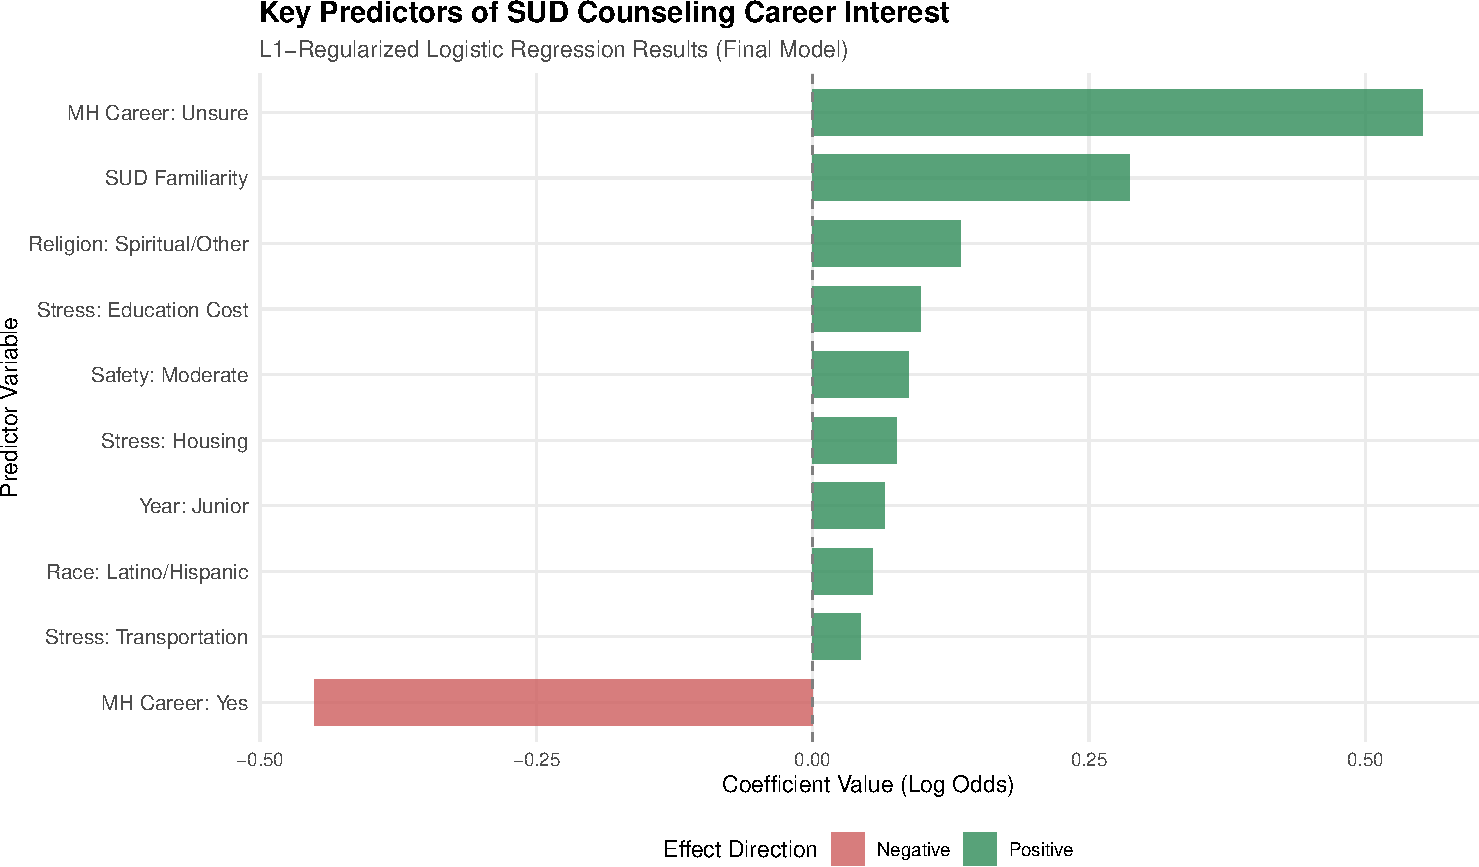
\includegraphics[keepaspectratio]{sud_council_paper_files/figure-pdf/fig-feature-importance-1.pdf}}

}

\end{figure}%

\textbf{Secondary Predictive Factors.} Beyond the primary mental health
career interest findings, one additional statistically robust pattern
emerged (Figure~\ref{fig-feature-importance}). Professional familiarity
with SUD counseling showed strong positive association (OR = 1.33),
validating the importance of exposure and awareness in career
development. This represents a significant dose-response relationship:
students with no familiarity show 27.6\% interest, while those with
moderate familiarity show 56.1\% interest (χ² = 16.64, p \textless{}
0.001). Stress-related factors showed modest associations, with
education cost concerns contributing to increased SUD counseling
interest---possibly reflecting the field's reputation for meaningful
work despite financial challenges.

\textbf{Academic and Developmental Patterns.} Early academic timing
showed meaningful associations, with first-year students demonstrating
highest interest (40.3\%, N=211) and second-year students maintaining
substantial interest (33.5\%, N=158). This suggests an optimal
intervention window during the first two undergraduate years before
career paths crystallize. Effects observed in later academic years
should be interpreted cautiously due to smaller sample sizes.

Final model hyperparameters were optimized through tidymodels grid
search: penalty λ = 0.0032, mixture α = 1.0 (pure Lasso), with SMOTE
upsampling for class balance. The complete tidymodels workflow and
detailed results are available in the project repository.

\subsubsection{Study 2: Focus Group Text
Analysis}\label{study-2-focus-group-text-analysis}

\textbf{Participants.} Seven focus group discussions were conducted with
undergraduate students (N=19 participants) to explore qualitative
perspectives on SUD counseling careers. Focus groups were designed to
capture diverse student perspectives and included both students with and
without prior mental health career interest.

\textbf{Procedure.} Focus groups lasted approximately 60-90 minutes and
were conducted via Zoom with video and audio recording. Discussions
explored: (1) students' understanding of SUD counseling as a profession,
(2) perceived barriers and facilitators to entering the field, (3)
career decision-making factors, (4) experiences with mental health and
substance use contexts, and (5) exploration of the career uncertainty
findings from Study 1.

\textbf{Text Analysis Approach.} Following supervised machine learning
for text analysis principles (\citeproc{ref-hvitfeldt2021}{Hvitfeldt \&
Silge, 2021}), we implemented a comprehensive preprocessing pipeline
using the tidytext framework (\citeproc{ref-silge2017}{Silge \&
Robinson, 2017}) and smltar methodology
(\citeproc{ref-hvitfeldt2021}{Hvitfeldt \& Silge, 2021}). This approach
allowed for systematic, reproducible analysis of focus group transcripts
while maintaining methodological rigor.

\textbf{Preprocessing Pipeline.} The analysis followed a five-stage
preprocessing approach: (1) \textbf{Tokenization} using
\texttt{unnest\_tokens()} for word-level analysis, (2) \textbf{Stopword
removal} from multiple sources (tidytext, custom focus group terms), (3)
\textbf{Porter stemming} using SnowballC to reduce words to root forms,
(4) \textbf{SUD term detection} using a comprehensive taxonomy of
substance-related terminology, and (5) \textbf{Utterance-level
classification} to identify SUD-relevant content.

\textbf{SUD Terminology Development.} We developed a comprehensive
taxonomy of 53 SUD-related terms organized into five categories: (1)
\textbf{Core Addiction Terms} (substance, addiction, dependence, etc.),
(2) \textbf{Specific Substances} (alcohol, drugs, opioids, etc.), (3)
\textbf{Treatment/Recovery} (recovery, therapy, counseling, etc.), (4)
\textbf{Problem Framing} (abuse, struggle, battle, etc.), and (5)
\textbf{Professional Context} (counselor, therapist, clinical, etc.).
All terms were systematically stemmed to ensure comprehensive detection
of word variations.

\textbf{Conservative Detection Approach.} Following methodological
validation, we implemented a conservative approach requiring the
presence of substance-specific terms (categories 1-2) to classify
utterances as SUD-relevant. This approach eliminated general mental
health discussions that lacked explicit substance use context, ensuring
precise focus on SUD counseling discourse. The final analysis included
61 utterances (19.7\% of substantive content) meeting conservative
SUD-relevance criteria.

\section{Results}\label{results}

\subsection{Study 1: Quantitative Analysis
Results}\label{study-1-quantitative-analysis-results}

The L1-regularized logistic regression analysis successfully identified
key predictors of SUD counseling career interest with strong predictive
performance and theoretical interpretability. Results demonstrate both
statistical significance and practical meaningful effect sizes for
behavioral prediction research.

\subsection{Study 2: Focus Group Text Analysis
Results}\label{study-2-focus-group-text-analysis-results}

\textbf{Overview of SUD-Relevant Discourse.} Analysis of focus group
transcripts identified 61 utterances (19.7\% of substantive content)
containing explicit substance use disorder terminology. This
conservative detection approach ensured that only discussions with clear
SUD context were included, avoiding general mental health conversations
that could introduce conceptual ambiguity.

\textbf{Thematic Co-occurrence Analysis.} We analyzed the most frequent
terms appearing alongside SUD discussions to identify dominant
conceptual themes. This approach revealed how students linguistically
frame and understand SUD counseling as a career option, providing
insight into the cognitive frameworks underlying career interest.

\subsubsection{Primary Thematic
Findings}\label{primary-thematic-findings}

\textbf{Personal-Emotional Framework (222 mentions, 36.8\% of SUD
discourse).} The most prominent theme centered on personal and emotional
processing, with ``feel'' (83 mentions) and ``family'' (30 mentions)
representing dominant co-occurring terms. Students consistently
discussed SUD counseling through personal experience lenses, suggesting
that career interest is mediated by emotional connection and lived
experience rather than purely academic or professional considerations
(see Table 3).

---INSERT TABLE 3 ABOUT HERE---

\textbf{People-Centered Orientation (202 mentions, 33.4\% of SUD
discourse).} Students consistently conceptualized SUD counseling through
relational frameworks, with ``people'' (83 mentions) dominating the
discourse. Additional relationship-focused terms included ``person'' (38
mentions) and family/friend references, indicating that students
understand SUD counseling primarily as people-focused helping work
rather than technical or clinical intervention.

\textbf{Professional Field Recognition (106 mentions, 17.5\% of SUD
discourse).} Students demonstrated clear recognition of SUD counseling
as a distinct professional field, with frequent mentions of ``field''
(29 mentions), ``job'' (25 mentions), and ``career'' (15 mentions). This
validates the Study 1 finding about career uncertainty as a recruitment
pathway---students conceptualize SUD counseling as a legitimate
professional option worthy of career consideration.

\textbf{Service-Helping Identity (140 mentions, 23.2\% of SUD
discourse).} Students strongly associated SUD counseling with helping
and service orientations, mentioning ``helping'' (33 mentions),
``counselor'' (27 mentions), and ``support'' (23 mentions). This theme
directly connects to Study 1's finding that students drawn to helping
professions show elevated SUD counseling interest.

\subsubsection{Methodological
Documentation}\label{methodological-documentation}

The text analysis followed a rigorous five-stage preprocessing pipeline
to ensure methodological validity and reproducibility (see Table 4). Our
comprehensive SUD terminology taxonomy organized 53 terms into five
distinct categories, providing systematic coverage of substance use
disorder discourse (see Table 5). The complete thematic analysis
revealed six major conceptual themes in student discussions of SUD
counseling careers (see Table 6).

---INSERT TABLE 4 ABOUT HERE---

---INSERT TABLE 5 ABOUT HERE---

---INSERT TABLE 6 ABOUT HERE---

\subsubsection{Integration with Study 1
Findings}\label{integration-with-study-1-findings}

\textbf{Career Uncertainty Pathway Validation.} The focus group analysis
provides qualitative support for Study 1's career uncertainty finding.
Students frequently discussed SUD counseling as a field they were
``exploring'' or ``learning about,'' consistent with the quantitative
finding that uncertain students show higher SUD interest. The
personal-emotional framing suggests that career uncertainty creates
openness to fields that resonate with personal experience.

\textbf{Familiarity and Exposure Mechanisms.} The prominence of family
and personal experience themes validates Study 1's familiarity effect
(OR = 1.33). Students with family members in helping professions or
personal exposure to substance use contexts demonstrated deeper
engagement with SUD counseling concepts, supporting targeted exposure
interventions.

\textbf{Professional Identity Formation.} The clear recognition of SUD
counseling as a distinct professional field supports recruitment
strategies that emphasize career legitimacy and professional development
opportunities. Students demonstrated sophisticated understanding of SUD
counseling as a specialized helping profession rather than a general
mental health role.

\section{Discussion}\label{discussion}

\subsection{Study 1: Implications for SUD Workforce
Development}\label{study-1-implications-for-sud-workforce-development}

\textbf{Mental Health Career Exploration as a Critical Pathway.} The
most significant finding concerns the relationship between mental health
career uncertainty and SUD counseling interest. Students who are
``Unsure'' about mental health careers show 74\% higher odds of SUD
counseling interest, while those already committed to mental health
careers show 36\% lower odds. This pattern suggests that \textbf{SUD
counseling serves as an important exploration and specialization
pathway} rather than competing directly with established mental health
career tracks.

This finding has immediate implications for recruitment strategy. Rather
than targeting students already committed to traditional mental health
careers (who may view SUD counseling as a departure from their plans),
efforts should focus on students in the career exploration
phase---particularly those expressing interest in helping professions
but uncertain about specific mental health specializations. This
represents a substantial and previously under-recognized recruitment
opportunity.

\textbf{Professional Familiarity and Exposure Effects.} The strong
positive association between SUD counselor familiarity and career
interest (OR = 1.33) validates the importance of awareness and exposure
in career development. This suggests that increasing visibility of the
SUD counseling profession---through coursework, guest speakers,
internship opportunities, or mentorship programs---could meaningfully
impact recruitment outcomes.

\textbf{Methodological Considerations and Effect Sizes.} The analysis
demonstrates strong statistical power for the primary findings, with the
mental health career interest effect achieving p \textless{} 0.001 (χ² =
92.59) and the familiarity effect reaching p \textless{} 0.001 (χ² =
16.64). These represent robust, replicable patterns unlikely to be due
to sampling variation. Demographic associations, while observed in the
model, did not reach statistical significance when tested independently
and should be interpreted cautiously given potential for Type I error in
multiple comparisons.

\textbf{Methodological Contributions.} This study demonstrates the value
of comprehensive variable preprocessing and strategic demographic
grouping in student survey research. The tidymodels implementation
provides a robust, reproducible framework for similar workforce
development research across helping professions.

\textbf{Broader Implications for Mental Health Workforce Development.}
These findings challenge traditional recruitment approaches that broadly
target students interested in mental health careers. Instead, results
suggest that \textbf{uncertainty represents opportunity}---students
still exploring their career options within mental health may be more
receptive to SUD counseling information and experiences than those
already committed to other specializations. This insight has immediate
applications for curriculum design, where SUD content might be most
effectively integrated into general mental health courses rather than
advanced specialty tracks.

\textbf{Policy and Educational Recommendations.} Based on the
statistically robust findings, workforce development initiatives should
prioritize: (1) \textbf{Early undergraduate interventions} during the
first two academic years when career exploration is optimal, (2)
\textbf{Systematic exposure programs} that increase familiarity with the
SUD counseling profession through coursework, guest speakers, and
experiential learning, and (3) \textbf{Targeted outreach} to students
expressing uncertainty about mental health career paths rather than
those already committed to other specializations. Educational
institutions should consider developing ``exploration tracks'' that
allow uncertain students to experience multiple mental health
specializations, including SUD counseling, before committing to specific
career paths.

\subsection{Study 2: Implications for Understanding SUD Career
Interest}\label{study-2-implications-for-understanding-sud-career-interest}

\textbf{Personal-Experiential Pathway to Career Interest.} The dominance
of personal-emotional frameworks in SUD discourse (36.8\% of SUD-related
content) provides critical insight into how students conceptualize SUD
counseling careers. Unlike technical or academic career orientations,
students approach SUD counseling through lived experience and emotional
connection. This suggests that recruitment messaging emphasizing
personal growth, meaningful work, and the opportunity to help others
facing similar challenges may be more effective than traditional
professional development appeals.

\textbf{Validation of Quantitative Findings Through Linguistic
Analysis.} Study 2 provides robust qualitative validation for Study 1's
key findings. The prominence of people-centered orientations (33.4\% of
discourse) validates the helping profession pathway identified
quantitatively. The clear professional field recognition (17.5\% of
discourse) supports the career uncertainty finding---students view SUD
counseling as a legitimate professional option worthy of exploration
rather than a secondary choice.

\textbf{Methodological Innovation in Mixed-Methods Research.} The
integration of supervised machine learning text analysis with focus
group methodology represents a significant methodological contribution.
By applying rigorous computational linguistics techniques to qualitative
data, we achieved systematic, reproducible thematic analysis while
maintaining the rich contextual insights characteristic of qualitative
research. The conservative detection approach (requiring
substance-specific terminology) ensures conceptual precision and
eliminates potential contamination from general mental health
discussions.

\textbf{Implications for Career Development Theory.} The thematic
patterns reveal that SUD counseling career interest develops through a
distinctive pathway combining personal experience, emotional processing,
and professional identity formation. This differs from traditional
career development models that emphasize skills, interests, and values
assessment. For SUD counseling, career interest appears to emerge from
the intersection of personal experience and recognition of professional
helping opportunities, suggesting that recruitment strategies should
address both emotional readiness and professional preparation.

\textbf{Targeted Intervention Opportunities.} The specific linguistic
patterns identified suggest precise intervention points for workforce
development. The prominence of family and personal experience themes
indicates that students with lived experience represent a crucial
recruitment population. The helping orientation emphasis suggests that
service-learning opportunities and volunteer experiences in SUD contexts
could effectively convert interest into career commitment. The
professional field recognition validates the importance of career
information and exposure programs.

\subsection{Limitations}\label{limitations}

\textbf{Sample Characteristics and Generalizability.} This study was
conducted at a single state university with a primarily undergraduate
population, which may limit generalizability to other institutional
contexts, graduate students, or students already enrolled in mental
health programs. The sample, while diverse, was drawn from a research
participation pool that may not fully represent the broader student
population's career interests and decision-making processes.

\textbf{Cross-Sectional Design.} The cross-sectional nature of Study 1
limits causal inferences about the relationship between predictors and
SUD counseling interest. Career interests may change over time, and
longitudinal research would provide stronger evidence for developmental
patterns and the stability of identified predictors.

\textbf{Career Interest vs.~Career Choice.} This study measured
expressed interest in SUD counseling rather than actual career choice or
persistence in the field. The relationship between early career interest
and eventual workforce entry may be moderated by additional factors not
captured in this analysis, including educational opportunities, job
market conditions, and personal circumstances.

\textbf{Measurement Considerations.} While the study achieved strong
predictive performance, some important constructs may have been
incompletely measured. For example, the mental health career interest
variable, while predictive, may not fully capture the complexity of
students' career development processes or their understanding of
different mental health specializations.

\textbf{Missing Variables.} Despite the comprehensive variable set,
important predictors of career interest may not have been included in
the survey, such as prior personal or family experiences with substance
use treatment, exposure to addiction coursework, or detailed
understanding of SUD counselor roles and responsibilities.

\section{References}\label{references}

\phantomsection\label{refs}
\begin{CSLReferences}{1}{0}
\bibitem[\citeproctext]{ref-hvitfeldt2021}
Hvitfeldt, E., \& Silge, J. (2021). \emph{Supervised machine learning
for text analysis in r}. Chapman; Hall/CRC. \url{https://smltar.com/}

\bibitem[\citeproctext]{ref-kuhn2020tidymodels}
Kuhn, M., \& Silge, J. (2022). \emph{Tidy modeling with r}. O'Reilly
Media. \url{https://www.tmwr.org/}

\bibitem[\citeproctext]{ref-silge2017}
Silge, J., \& Robinson, D. (2017). \emph{Text mining with r: A tidy
approach}. O'Reilly Media. \url{https://www.tidytextmining.com/}

\end{CSLReferences}

\appendix

\subsection{Variable Descriptions}\label{variable-descriptions}

\begin{longtable}[]{@{}
  >{\raggedright\arraybackslash}p{(\linewidth - 4\tabcolsep) * \real{0.1164}}
  >{\raggedright\arraybackslash}p{(\linewidth - 4\tabcolsep) * \real{0.8147}}
  >{\raggedright\arraybackslash}p{(\linewidth - 4\tabcolsep) * \real{0.0690}}@{}}
\toprule\noalign{}
\begin{minipage}[b]{\linewidth}\raggedright
Variable
\end{minipage} & \begin{minipage}[b]{\linewidth}\raggedright
Description
\end{minipage} & \begin{minipage}[b]{\linewidth}\raggedright
Type
\end{minipage} \\
\midrule\noalign{}
\endhead
\bottomrule\noalign{}
\endlastfoot
Progress & The variable `Progress' measures the percentage of completion
or advancement in a given task or project, represented as a numerical
value from 0 to 100. & Numeric \\
Duration (in seconds) & This variable measures the duration of an event
or activity in seconds, capturing how long it takes to complete a
specific task. & Numeric \\
CarelessResponderDC & This variable indicates whether a respondent
completed the survey in less than the threshold duration of 120 seconds,
with a value of 1 signifying a potentially careless response. &
Categorical \\
Finished & The variable `Finished' indicates whether a task or activity
has been completed, with a binary response of either completed (True) or
not completed (False). & Categorical \\
RecordedDate & The RecordedDate variable captures the date and time when
a particular event or response was logged, providing a timestamp for
data collection. & Other \\
ResponseId & Response ID is a unique identifier assigned to each survey
response, allowing for tracking and analysis of individual submissions.
& Text \\
Q46 & This variable measures the consent status of participants
regarding their age and willingness to participate in the research
study. & Categorical \\
demo\_age & This variable measures the age of respondents in years,
capturing a range of age groups and preferences regarding age
disclosure. & Categorical \\
demo\_gender & This variable measures the gender identity of
respondents, capturing their self-identification in terms of gender. &
Categorical \\
demo\_sex & This variable measures the sex assigned to an individual at
birth, reflecting their biological classification. & Categorical \\
demo\_country & This variable captures the country of birth of the
survey respondent, providing insights into demographic backgrounds. &
Categorical \\
demo\_race & This variable captures the racial identity of respondents
as part of demographic data collection. & Categorical \\
demo\_race\_7\_TEXT & This variable captures the self-reported race of
respondents who selected `Other' in a survey, allowing for open-ended
text responses to specify their racial identity. & Text \\
demo\_served & This variable measures whether an individual has ever
served on active duty in the U.S. Armed Forces, indicating their
military service status. & Categorical \\
demo\_disability & This variable measures whether an individual has a
formally diagnosed disability as recognized by a medical professional. &
Categorical \\
demo\_schoolyear & This variable measures the current year in school of
the respondents, indicating their level of progression in their
educational journey. & Categorical \\
demo\_parenteducation & This variable measures the highest level of
education completed by the respondent's parents or guardians, reflecting
their educational background. & Categorical \\
demo\_employment & This variable measures the current employment
situation of respondents, capturing whether they are employed,
unemployed, or in school with varying work hours. & Categorical \\
demo\_housing & The variable measures the current living situation of
respondents while attending Binghamton University, indicating whether
they reside on-campus, off-campus, or with family. & Categorical \\
demo\_livewith & This variable measures the total number of friends or
family members living with the respondent at their current residence
while attending school. & Numeric \\
demo\_safety & This variable measures the respondents' perception of
their physical safety in their neighborhood while attending school. &
Categorical \\
demo\_permanenthome & This variable measures the type of permanent
residence of the respondent when not attending school, indicating their
living situation. & Categorical \\
demo\_permanenthome\_5\_TEXT & This variable captures the description of
the respondent's permanent residence when not attending school, allowing
for open-ended responses. & Text \\
demo\_geography & This variable measures the type of geographic area in
which the respondent grew up, categorizing their upbringing into
distinct environments. & Categorical \\
demo\_safeathome & This variable measures the respondent's perception of
physical safety in their childhood neighborhood, reflecting their
feelings of security during that time. & Categorical \\
demo\_caregiver & This variable measures whether the respondent serves
as a caregiver for individuals aged 18 or older. & Categorical \\
demo\_familyincome & This variable measures the annual household income
of respondents, capturing the combined income of all individuals living
in their home or permanent residence. & Categorical \\
demo\_personalincome & This variable measures the respondent's personal
annual income, capturing a range of income levels as well as options for
non-disclosure. & Categorical \\
demo\_religion & This variable measures the respondent's religious
affiliation or beliefs, capturing their identification with specific
religious branches or lack thereof. & Categorical \\
demo\_addiction & This variable measures whether an individual has ever
been diagnosed or treated for a substance use or addiction concern,
providing insight into their personal history with addiction. &
Categorical \\
demo\_familyaddiction & This variable measures whether a respondent has
a close friend or family member who has been diagnosed or treated for a
substance use or addiction concern, indicating the prevalence of
addiction issues within personal networks. & Categorical \\
demo\_mentalhealth & This variable measures whether an individual has
ever been diagnosed or treated for a mental health concern, indicating
their mental health history. & Categorical \\
demo\_people & This variable measures the frequency with which
individuals engage in social interactions with people they care about,
reflecting their social connectivity and support network. &
Ordinal/Likert \\
demo\_anythingelse & This variable captures additional information about
the respondent's background that may not be covered by other survey
questions, allowing for open-ended responses. & Text \\
career\_1 & This variable measures the respondent's level of familiarity
with the substance use disorder counselor profession, ranging from no
familiarity to a high degree of familiarity. & Ordinal/Likert \\
career\_2 & This variable measures the respondent's level of interest in
pursuing a career as a substance use disorder counselor. &
Ordinal/Likert \\
career\_4\_1 & This variable measures the ranked importance of various
reasons for interest in becoming a substance use disorder counselor,
focusing on personal motivations and values. & Ordinal/Likert \\
career\_4\_2 & This variable measures the ranked importance of various
reasons for interest in becoming a substance use disorder counselor,
specifically focusing on the second reason selected by respondents. &
Ordinal/Likert \\
career\_4\_3 & This variable measures the ranked importance of various
reasons for interest in becoming a substance use disorder counselor,
focusing on personal motivations and values. & Ordinal/Likert \\
career\_6\_1 & This variable measures the ranked importance of factors
that influence the interest in pursuing a career as a substance use
disorder counselor, with respondents identifying their top three
priorities. & Ordinal/Likert \\
career\_6\_2 & This variable measures the ranked importance of factors
that could make a career as a substance use disorder counselor more
appealing or feasible for respondents. & Text \\
career\_6\_3 & This variable captures the ranked preferences of
respondents regarding factors that would enhance the appeal or
feasibility of a career as a substance use disorder counselor. & Text \\
career\_5\_1 & This variable captures the top three reasons respondents
are not interested in pursuing a career as a substance use disorder
counselor, ranked by importance. & Text \\
career\_5\_2 & This variable captures the top three reasons respondents
are not interested in pursuing a career as a substance use disorder
counselor, reflecting personal motivations and barriers. & Text \\
career\_5\_3 & This variable captures the top three reasons respondents
are not interested in pursuing a career as a substance use disorder
counselor, reflecting personal attitudes and experiences related to the
field. & Text \\
career\_3 & This variable measures the respondent's awareness of
individuals who have worked or are currently working as substance use
disorder counselors. & Categorical \\
career\_3fu & This variable measures the relationships of respondents to
individuals who have worked or are currently working as substance use
disorder counselors, capturing personal connections such as family
members or friends. & Text \\
mh\_1 & This variable measures the respondent's interest in pursuing a
career in mental health counseling or related fields. & Categorical \\
mh\_4 & This variable measures the areas of specialization that
respondents are interested in pursuing if they were to become a mental
health counselor, allowing for multiple selections. & Categorical \\
mh\_4\_12\_TEXT & This variable captures the areas of specialization
that respondents are interested in pursuing if they were to become
mental health counselors, specifically focusing on `other' specialties
that are not listed in predefined options. & Text \\
mh\_1.5 & This variable captures the various classes and training
experiences that respondents believe are necessary for individuals to
become mental health counselors or therapists. & Text \\
Q44 & This variable captures the names and titles of degree programs
that respondents associate with becoming a mental health counselor,
reflecting their perceptions of relevant educational pathways. & Text \\
Q45 & This variable measures respondents' perceptions of the duration
required to become a mental health counselor, reflecting their
understanding of the training and education involved. & Categorical \\
Q46.1 & This variable measures the perceived cost of education or
training required to become a mental health counselor, capturing a range
of monetary values and uncertainty. & Categorical \\
Q47 & This variable measures the preferred location for attending a
training program in mental health counseling among respondents. &
Categorical \\
mh\_3fu & This variable captures the reasons respondents prefer a
specific location, reflecting their personal experiences and motivations
related to that location. & Text \\
wellbeing\_1 & This variable measures the level of concern or stress
individuals experience regarding education-related expenses, capturing
their subjective feelings about this financial issue. &
Ordinal/Likert \\
wellbeing\_2 & This variable measures the level of concern or stress
individuals experience regarding the cost of housing. &
Ordinal/Likert \\
wellbeing\_3 & This variable measures the level of concern or stress
related to the stability of housing, as reported by respondents. &
Ordinal/Likert \\
wellbeing\_4 & This variable measures the level of concern or stress
individuals experience regarding the cost of groceries. &
Ordinal/Likert \\
wellbeing\_5 & The variable measures the level of concern or stress
individuals experience regarding the cost of transportation. &
Ordinal/Likert \\
wellbeing\_6 & This variable measures the level of concern or stress
individuals experience regarding the reliability of transportation. &
Ordinal/Likert \\
wellbeing\_7 & This variable measures the level of concern or stress
individuals experience regarding access to high-speed internet. &
Ordinal/Likert \\
wellbeing\_8 & This variable measures the level of concern or stress
individuals experience regarding the cost of childcare. &
Ordinal/Likert \\
wellbeing\_9 & This variable measures the level of concern or stress
individuals experience regarding access to childcare. &
Ordinal/Likert \\
wellbeing\_10 & The variable measures the level of concern or stress
individuals feel regarding the stability and safety of their
relationships with people they currently live with. & Ordinal/Likert \\
\end{longtable}

\section{Tables}\label{tables}

\begin{table}

{\caption{{Table 3. Personal-Emotional Framework: Top Co-occurring Terms
in SUD Discussions}{\label{tbl-study2-personal-theme}}}
\vspace{-20pt}}

\begin{longtable}[]{@{}lrr@{}}
\toprule\noalign{}
Term & Frequency & Percentage of SUD Discourse \\
\midrule\noalign{}
\endhead
\bottomrule\noalign{}
\endlastfoot
feel & 83 & 13.8 \\
family & 30 & 5.0 \\
life & 17 & 2.8 \\
experience & 14 & 2.3 \\
friends & 15 & 2.5 \\
emotions & 13 & 2.2 \\
stories & 5 & 0.8 \\
\end{longtable}

\end{table}

\begin{table}

{\caption{{Table 4. Text Preprocessing Pipeline Following
smltar/tidytext Methodology}{\label{tbl-study2-preprocessing-pipeline}}}
\vspace{-20pt}}

\begin{longtable}[]{@{}
  >{\raggedright\arraybackslash}p{(\linewidth - 8\tabcolsep) * \real{0.0420}}
  >{\raggedright\arraybackslash}p{(\linewidth - 8\tabcolsep) * \real{0.1933}}
  >{\raggedright\arraybackslash}p{(\linewidth - 8\tabcolsep) * \real{0.3193}}
  >{\raggedright\arraybackslash}p{(\linewidth - 8\tabcolsep) * \real{0.2269}}
  >{\raggedright\arraybackslash}p{(\linewidth - 8\tabcolsep) * \real{0.2185}}@{}}
\toprule\noalign{}
\begin{minipage}[b]{\linewidth}\raggedright
Step
\end{minipage} & \begin{minipage}[b]{\linewidth}\raggedright
Process
\end{minipage} & \begin{minipage}[b]{\linewidth}\raggedright
Method
\end{minipage} & \begin{minipage}[b]{\linewidth}\raggedright
Input
\end{minipage} & \begin{minipage}[b]{\linewidth}\raggedright
Output
\end{minipage} \\
\midrule\noalign{}
\endhead
\bottomrule\noalign{}
\endlastfoot
1 & Tokenization & tidytext::unnest\_tokens() word-level & 310
substantive utterances & 20,890 raw tokens \\
2 & Stopword Removal & Multi-source stopwords + custom terms & 20,890
raw tokens & 4,324 meaningful tokens \\
3 & Stemming & Porter stemming via SnowballC & 4,324 tokens & 1,000
unique stems \\
4 & SUD Term Processing & Apply stemming to 53 SUD terms & 53 original
terms & 42 unique stems \\
5 & Conservative Detection & Require substance-specific terms & 310
total utterances & 61 SUD utterances (19.7\%) \\
\end{longtable}

\end{table}

\begin{table}

{\caption{{Table 5. SUD Terminology Taxonomy: Categories and Examples
Used for Text Detection}{\label{tbl-study2-methodology-table}}}
\vspace{-20pt}}

\begin{longtable}[]{@{}
  >{\raggedright\arraybackslash}p{(\linewidth - 6\tabcolsep) * \real{0.2211}}
  >{\raggedleft\arraybackslash}p{(\linewidth - 6\tabcolsep) * \real{0.1263}}
  >{\raggedright\arraybackslash}p{(\linewidth - 6\tabcolsep) * \real{0.3474}}
  >{\raggedright\arraybackslash}p{(\linewidth - 6\tabcolsep) * \real{0.3053}}@{}}
\toprule\noalign{}
\begin{minipage}[b]{\linewidth}\raggedright
Category
\end{minipage} & \begin{minipage}[b]{\linewidth}\raggedleft
Terms\_Count
\end{minipage} & \begin{minipage}[b]{\linewidth}\raggedright
Example\_Terms
\end{minipage} & \begin{minipage}[b]{\linewidth}\raggedright
Stemmed\_Examples
\end{minipage} \\
\midrule\noalign{}
\endhead
\bottomrule\noalign{}
\endlastfoot
Core Addiction & 8 & substance, addiction, dependence & substanc,
addict, depend \\
Specific Substances & 13 & alcohol, drug, opioid & alcohol, drug,
opioid \\
Treatment/Recovery & 17 & recovery, therapy, counseling & recoveri,
therapi, counsel \\
Problem Framing & 8 & abuse, struggle, battle & abus, struggl, battl \\
Professional Context & 7 & counselor, therapist, clinical & counselor,
therapist, clinic \\
\end{longtable}

\end{table}

\begin{table}

{\caption{{Table 6. Complete Thematic Analysis: Word Co-occurrence
Patterns in SUD Discourse}{\label{tbl-study2-thematic-summary}}}
\vspace{-20pt}}

\begin{longtable}[]{@{}
  >{\raggedright\arraybackslash}p{(\linewidth - 8\tabcolsep) * \real{0.1795}}
  >{\raggedleft\arraybackslash}p{(\linewidth - 8\tabcolsep) * \real{0.1111}}
  >{\raggedleft\arraybackslash}p{(\linewidth - 8\tabcolsep) * \real{0.1282}}
  >{\raggedleft\arraybackslash}p{(\linewidth - 8\tabcolsep) * \real{0.2137}}
  >{\raggedright\arraybackslash}p{(\linewidth - 8\tabcolsep) * \real{0.3675}}@{}}
\toprule\noalign{}
\begin{minipage}[b]{\linewidth}\raggedright
Theme
\end{minipage} & \begin{minipage}[b]{\linewidth}\raggedleft
Unique\_Stems
\end{minipage} & \begin{minipage}[b]{\linewidth}\raggedleft
Total\_Mentions
\end{minipage} & \begin{minipage}[b]{\linewidth}\raggedleft
Percentage\_SUD\_Discourse
\end{minipage} & \begin{minipage}[b]{\linewidth}\raggedright
Top\_Terms
\end{minipage} \\
\midrule\noalign{}
\endhead
\bottomrule\noalign{}
\endlastfoot
Personal-Emotional & 10 & 222 & 36.8 & feel (83), family (30), life
(17) \\
People-Relationships & 12 & 202 & 33.4 & people (83), person (38),
friends (15) \\
Service-Helping & 10 & 140 & 23.2 & helping (33), counselor (27),
support (23) \\
Professional Field & 8 & 106 & 17.5 & field (29), job (25), career
(15) \\
Challenge-Barrier & 6 & 39 & 6.5 & hard (17), struggling (10), issue
(5) \\
Interest-Motivation & 5 & 13 & 2.2 & compassionate (4), enjoy (3),
appeal (2) \\
\end{longtable}

\end{table}






\end{document}
